%%%%%%%%%%%%%%%%%%%%%%%%%%%%%%%%%%%%%%%%%%%%%%%%%%%%%%%%%%%%
%%%%%%%%%%%%%%%%%%%%%%%%%%%%%%%%%%%%%%%%%%%%%%%%%%%%%%%%%%%%
\chapter{Characterization of Phenomenological Spectral Distributions}
\label{chap:db}
\nopagebreak
%%%%%%%%%%%%%%%%%%%%%%%%%%%%%%%%%%%%%%%%%%%%%%%%%%%%%%%%%%%%
%%%%%%%%%%%%%%%%%%%%%%%%%%%%%%%%%%%%%%%%%%%%%%%%%%%%%%%%%%%%

A Tandem Mass Spectrometry product is represented by a list of measured
mass-to-charge $m/z$ ratio of the ions that are observed during the measurement.
Those values are accompanied by an intensity which is directly proportional to
the number of ions observed.
Generally the spectrum comes with further information due to the MS$_1$ spectrum: the
precursor ion mass $MH^+$ and the precursor ion charge $Q$.
Moreover the product ion peaks come mixed to instrument noise, isotopes and
other puzzling signals 
that complicate the task of assigning each peak to a product ion.

The absolute intensity of a spectrum is mainly related to the amount of
precursor peptide in the sample, so that it does not provide useful information
for identification. However different kind of product peaks present generally
different intensities
and different ratios with other ion types.
Generally $b$ and $y$ ions present higher intensity compared to the others.
Noise peaks are usually considered to present lower intensity.

Knowing the exact distribution of each ion type in the $(\frac m z,I)$ plane we can
infer the probability of a peak to belong to one type of product ion or
another, or to the noise.

Thus our strategy, and the objective of this chapter, is to learn the distribution of
the different families of peaks from a database of spectra for which a reliable
interpretation has been provided. 
Using this information we will derive in Chapter~\ref{chap:pot} an
energy function for the unidimensional statistical-mechanics model presented in
chapter \ref{chap:alg} to infer the precursor
peptide sequence from the peaks observed in the experimental spectrum.


%+++++++++++++++++++++++++++++++++++++++++++++++++++++++++++++++++++++++++++
\section{Building the learning database}
%+++++++++++++++++++++++++++++++++++++++++++++++++++++++++++++++++++++++++++

%+++++++++++++++++++++++++++++++++++++++++++++++++++++++++++++++++++++++++++
\subsection{Preliminary choice of the spectra}
%+++++++++++++++++++++++++++++++++++++++++++++++++++++++++++++++++++++++++++

%We collected a learning set of peaks from different spectra. 
%The latter where extracted from freely available databases
%deposited on the web by different research groups.
We collected a learning set of peaks from different spectra. 
The latter where extracted from a freely available database
deposited on the web, and hosting the work of different research groups.
The website offering those data is available on the internet at the following
address:
%\begin{itemize}
%\item \href{http://bioinformatics.icmb.utexas.edu/OPD/}{http://bioinformatics.icmb.utexas.edu/OPD}
% from the University of Texas;
%\item 
\href{http://www.peptideatlas.org/}{www.peptideatlas.org} from the Seattle Proteome
Center.
%\end{itemize}

Those data where collected by different instruments and, in all the cases, they came
with the interpretation carried out by the database search algorithm SEQUEST.
The databases we have used are the followings, listed with the experimental
instrument employed:
%{\bf MAURO, magari da' un occhiata, anche senza scrivere niente qui, a che tipo di spettri vengono da ciascun strumento: hanno tutti le stesse caratteristiche? Magari te lo chiedono durante la  difesa, }
\begin{itemize}
% \item Open Proteomics Database:
% \begin{itemize}
%  \item opd00005\_ECOLI;
% \end{itemize}
% \item PeptideAtlas:
% \begin{itemize}
  \item PAe000032 \cite{schnapp2006mining} LCQ-DECA ion mass spectrometer
(Thermo-Finnigan) and a micro-electrospray source (Brechbuehler);
% SEQUEST sequencing has been verified by PeptideProphet and ProteinProphet;
  \item PAe000035 \cite{schnapp2006mining} LCQ-DECA (Thermo-Finnigan);
%  \item PAe000093 \cite{mackay2004gene} Integral HPLC;
%  \item PAe000096 \cite{omenn2004human}
  \item PAe000142 \cite{maynard2004characterizing} 2D HPLC coupled with the
classical LCQ-ESI ion trap (Thermo-Finnigan);
  \item PAe000219 \cite{goo2003proteomic} $\mu$LC-ESI-MS/MS using LCQ-DECA
(Thermo-Finnigan);
  \item PAe000244 \cite{goo2003proteomic} $\mu$LC-ESI-MS/MS using LCQ-DECA
(Thermo-Finnigan);
%  \item PAe000324 \cite{piening2006quality} nanoLC-MS/MS using a nanoflow HPLC from Agilent and a
%linear ion trap LCQ from Thermo-Finnigan;
%  \item PAe000071 -just for tests- \cite{omenn2004human} We don't have the paper
%(buy it?)
% \end{itemize}
\end{itemize}


%+++++++++++++++++++++++++++++++++++++++++++++++++++++++++++++++++++++++++++
\subsection{Filtering for spectra with a reliable interpretation}


In MS/MS, the sequence assignation through \emph{database search} algorithms like
SEQUEST or Mascot is affected by a significant number of false positives
\cite{keller2002experimental}, affecting peptide sequencing with incorrect
sequences.
There are a number of algorithms written to improve peptide scoring and to
better distinguish low quality sequence assignations from reliable ones. 
Some examples are: Protein
Prophet \cite{proteinprophet2002,aebersold2003statistical}, SEQUEST-NORM
\cite{yates-analchem-2002}, MASPIC \cite{narasimhan2005maspic}.
The selection of a reliable data set, from the published experimental data, is
then a central point in a database-learning schema.

\begin{table}[!thb]
\centering
\begin{tabular}{ccc}
\hline
\hline
q & XCorr cut-off & $\Delta C_n$ cut-off\\
\hline
1 & 1.5	& 0.3\\
2 & 3.0	& 0.3\\
3 & 3.5	& 0.3\\
\hline
\hline
\end{tabular}
\caption{\label{tab:xcorr-cutoff}The table reports cut-off values for XCorr and
$\Delta C_n$.
We filter MS/MS spectrometry databases based on these values to extract a set of
reliable spectra.
The XCorr cut-off value is correlated to the precursor charge, to avoid the
introduction of biases we choose different values for each charge state.}
\end{table}

The spectra of each set come with an associated SEQUEST score \emph{XCorr}.
This algorithm uses a cross correlation function to measure the quality of the
match between the tandem mass spectrum and an amino acid sequence selected from
a sequences database.
SEQUEST creates a model of the spectrum expected from the precursor peptide
represented by the sequence, relying on a simple interpretation of the CID
fragmentation. This ``theoretical spectrum'' is matched to the target spectrum
calculating the cross correlation between them.
The latter depends on the quality if the spectrum and on the quality of the
match with the theoretical one\cite{eng1994}.
On the other hand this score function depends also on the length of the peptide
considered as discussed by \citet{yates-analchem-2002}, where the authors
describe a improved score introducing a normalizing term defined as the cross
correlation of the target spectrum with itself, where the latter represents the best possible
match.

We want to extract from the downloaded databases a subset of spectra with
reliable sequence assignment and,
in order to assure the reliability of the sequence assignment, we introduce a
cut-off in the XCorr value, discarding low rated data more likely to be
incorrect matching.
Charge state of the precursor peptide depends on its length as longer ions are
more likely to carry an higher quantity of charge, then, in order to correct
XCorr bias, we use a different cut-off for each charge.

SEQUEST interpretation comes also with the measure $\Delta C_n$, a parameter that
represents how much the first ranked sequence is more probable compared with the second
ranked one.
We introduce, then, another threshold on the $\Delta C_n$ parameter: only
spectra whose interpretation has a $\Delta C_n$ higher then $0.3$ are accepted
(in \cite{yates1995mining,yates1995method} it
has been reported as acceptable a value of $0.1$).

Table \ref{tab:xcorr-cutoff} reports the selected cut-off values for XCorr and
$\Delta C_n$.

%+++++++++++++++++++++++++++++++++++++++++++++++++++++++++++++++++++++++++++
\subsection{Filtering over-represented precursor peptides}

The cell proteome can contain
thousands of different types of protein, with heterogeneous expression dynamic range.
Proteins expression is variable depending on the cell state and type.
During the cell life, different proteins can be expressed in different amounts, and
the number of copies of the same molecule can easily span 5 order of magnitude
\cite{aebersold2001mass}.
A single gene can express the same protein with a dynamic range of 4 order of magnitude
between the fully repressed and the fully induced state
\cite{finley2002regulated}.

\begin{figure}[!thb]
\begin{center}
\includegraphics[angle=-90,width=0.6\textwidth]{./img/msms/all-peptides-expression-dist.eps}\\
\caption{\label{fig:multi-copies}
Number of different peptides vs number of copies in the downloaded
databases.
The database presents a large number of copies of the same
peptide while the majority of the peptides just come in few copies.
Spectra are extracted from the downladed databases on the bases of the XCorr and
$\Delta C_n$ contraints, before the application of further filters.
There are 1.530.738 spectra from 1.021.431 different peptides.}
\end{center}
\end{figure}

The output databases of MS/MS spectroscopy experiments are composed of spectra
of different peptides which present multiple copies of itself, while other
peptides just came in very few copies.
Figure \ref{fig:multi-copies} reports the database dynamic
range: some peptides are expressed with thousands of copies while the majority
just came with few copies.

The presence of few peptides with such number of spectrum copies can invalidate a
distribution study. To avoid that the number of copies biases the
peaks distribution, we take into account only a maximum number of 10 copies per
peptide.


\subsection{Filtering the Precursor Mass and Sequence Consistency}


Despite the available 
instrument sensibility, it is usual to find erroneous values of
the precursor mass, sometimes accountable to human data mis-interpretation of
the experimental data or parameter.
As shown in Fig.~\ref{fig:mh-dist}, the difference between the mass provided by
the instrument measure of the precursor peak and reported in the spectrum file
and the mass expected for the amino acid content of the precursor has a wide
distribution covering a range about 6 Da, in the database.
This is a source of confusion for the peak interpretation.
Notice that the actual distribution presents some peaks uniformly separated by 1
Da that suggests a erroneous selection of the mono-isotopic precursor peak in
the experimental procedure, see Subsec.~\ref{subsec:cid-spectrum} for a detailed
description.
\begin{figure}
\centering
\subfigure[tot]{
\includegraphics[width=2cm,angle=-90]{./img/msms/MH-dist-small-tot.eps}}
\subfigure[$Q=1$]{
\includegraphics[width=2cm,angle=-90]{./img/msms/MH-dist-small-q1.eps}}\\
\subfigure[$Q=2$]{
\includegraphics[width=2cm,angle=-90]{./img/msms/MH-dist-small-q2.eps}}
\subfigure[$Q=3$]{
\includegraphics[width=2cm,angle=-90]{./img/msms/MH-dist-small-q3.eps}}
\caption{\label{fig:mh-dist}
Precursor mass distribution as reported in the dta files of experimental data. The
reported value is the difference in mass between the value reported in the
experimental spectrum file and the mono-isotopic value calculated from the sequence
proposed by SEQUEST. The figure represent the total distribution (28085
precursor masses from the downloaded spectra, before the application of the
precursor mass constraint) (a), and the single distributions
accounting for precursors with 1 (b),2 (c) or 3 (c) charges respectively.}
\end{figure}

We introduce, then, a further constraint on the experimental precursor mass to be
consistent with the theoretical mass calculated from the sequence proposed by
SEQUEST. 
Here the theoretical mass of the sequence is the sum of the
mono-isotopic masses of the residues reported with the masses of the N-term, the
C-term and the additional hydrogen.
The two values of the theoretical and the experimental masses have to differ
less then 0.5 Da.

Finally in Table \ref{tab:num-spectra} we resume the resulting number of spectra
that respect all the constraints mentioned above and are considered
in this work as the learning database.

\begin{table}[!thb]
\begin{center}
\begin{tabular}{cc}
\hline
\hline
q & n. of spectra \\
\hline
%1&  1339  \\
%2&  19790 \\
%3&  8673  \\
1&  158  \\
2&  7839 \\
3&  1390  \\
\hline
\hline
\end{tabular}
\caption{\label{tab:num-spectra}
Number of spectra for different values of parent charge considered in the
learning database.
Each precursor ion is present with a maximum spectra number of 10, and respects
the mass constrain.}
\end{center}
\end{table}


%-----------------------------------------------------------------------------
\section{Peak Processing and Recognition}
%+++++++++++++++++++++++++++++++++++++++++++++++++++++++++++++++++++++++++++

Spectra in the dataset, which came in the SEQUEST data file format, are composed
by a list of pairs
$\{\pi_\alpha\equiv(\rho_\alpha,I_\alpha)\}$, where $\rho_\alpha$ represents the
$m/z$ ratio of the fragment ($m$ is expressed in atomic mass units) and $I_\alpha$ the
intensity of its peak, proportional to the ion count.
The list of peaks is completed with the information about the precursor-ion's mass $m(MH^+)$ and charge $Q$. The total mass of the precursor
ion refers to the mass of the corresponding single charged ion, including the
proton carrying the positive charge.


%A spectrum is a set peaks represented by couples of mass-charge ratio 
%($\rho=\frac m z$) and a peak intensity ($I$). The spectrum information is
%completed by the parent mass ($MH$) and its charge state ($Q$).
%
%\begin{itemize}
% \item[mass\_sequest] the mass provided by sequest naked of N and C-term;
% \item[mass\_mono] the sum of the aa mono isotopic masses (aa are provided by sequest sequence);
% \item[mass\_ave] the sum of the aa average masses;
% \item[MH] mass\_mono + N-term + C-term.
%\end{itemize}

%+++++++++++++++++++++++++++++++++++++++++++++++++++++++++++++++++++++++++++
\subsection{Removing Isotopes}
%+++++++++++++++++++++++++++++++++++++++++++++++++++++++++++++++++++++++++++

The vast variety of proteins contained in the living organisms is only composed
of few types of atoms combined in  the amino acid structures. The atomic content
of the 20 amino-acid vocabulary 
is composed by, mainly,
carbon (C), nitrogen (N), hydrogen (H) and oxygen (O), with a  lower
content of sulphur (S).

Those atoms naturally come with different number of neutrons (isotopes), but one can consider that
only carbon and nitrogen atoms present a non negligible probability to present
as isotope in a precursor ion.

\begin{table}[!thb]
\centering
\begin{tabular}{cc|cccc}
\hline
\hline
Element & Conc. ($Da^{-1}$) &  Isotope & N. A.&  Isotope & N. A.\\
\hline
C & 0.0436733471  & ${}^{13}C$  & 1,07 \%  \\%0.04446942
H & 0.0696327313  & ${}^{2}H$   & 0.015\%  \\
N & 0.0122689921  & ${}^{15}N$  & 0,364\%  \\%0.01222999
O & 0.0139260967  & ${}^{17}O$  & 0.039\% & $^{18}O$  & 0.201\% \\
S & 0.0003500522  & ${}^{33}S$  & 0.75 \% & $^{34}S$  & 4.21\%  \\
\hline
\hline
\end{tabular}
\caption{\label{tab:isotopes}
The 5 elements representing the basic constituents of the 20 amino acids, with
the expected concentration per mass unit in proteins (second column).
In nature these elements coexist with a fraction of stable isotopes, reported on
the following columns along with their natural abundance (N.A.).}
\end{table}

The presence of isotopes in MS/MS mass spectrometry results in multiplicity of
peaks corresponding to a single product ion with a typical distribution of peaks
at a distance of one Da., or fractions if the ion carry a charge $Q$ higher than
one.
This set of peaks, called the isotope peak train, is generally observed for the
highest peaks and for bigger ions. 
The first peak represents the
isotope-free ion composed only by $^{12}C$ and $^{14}N$, while
the following peaks represent ions with only one or only two isotopes and
so on.
A train of isotope peaks $\{\pi_\alpha,\alpha=i\dots j\}$ 
%is found if
between peaks 
$\pi_i$, $\pi_j$, is defined as a set of nearby peaks satisfying the conditions 
$\rho_\alpha-\rho_i\le0.2\cdot(\alpha-i) Da$, where absent peaks are not allowed.
The peak intensity represents the amount of identical ions detected, then
the relative intensity of the isotope peak $I_\alpha$ and
the mono-isotopic peak $I_i$ depends on the probability to find an
isotope-free fragment and the probability to find exactly $n$ isotopes as in the
following:
\begin{align}
 \frac{I_i}{I_\alpha} &= 
\frac{p(\mathcal N(^{13}C)=0)p(\mathcal N(^{15}N)=0)}
{\sum_{\sigma=0}^s \left(
p(\mathcal N(^{13}C)=\sigma)p(\mathcal N(^{15}N)=s-\sigma)
\right)}
\label{eq:isotope-int}\\
\intertext{where $\mathcal N(^x X)$ is the number of isotope $x$ of element
$X$ in the fragment considered, and:}
p(\mathcal N(^{13}C)=0)&=(1-p({^{13}C}))^{n_C}\\
p(\mathcal N(^{15}N)=0)&=(1-p({^{15}N}))^{n_N}\\
p(\mathcal N(^{13}C)=\sigma) &= \binom{n_C} \sigma
(p({^{13}C}))^\sigma (1-p({^{13}C}))^{n_C-\sigma}\\
p(\mathcal N(^{15}N)=s-\sigma)&= \binom{n_N}{s-\sigma}
(p({^{15}N}))^{s-\sigma}(1-p({^{15}N}))^{n_N-(s-\sigma)}
\end{align}
Here $s=(\alpha-i)$ and only isotopes with $s\le4$ are considered; % While 
$p({^n X})$ 
is the natural abundance of isotope $n$ of the element $X$, as in table
\ref{tab:isotopes}, and $n_X$ its the expected number of the element $X$
calculated from the mass-to-charge ratio $\rho$ of the peaks.

When a train of isotopes $\{\pi_\alpha,\alpha=i\dots j\}$ is detected in the
spectrum, we keep only the trailing isotope-free peak $\pi_i$ while peaks
containing isotopes are removed.

All the process is repeated for ions carrying a double charge, in the case
of precursor ions with charge higher than one.


%+++++++++++++++++++++++++++++++++++++++++++++++++++++++++++++++++++++++++++
\subsection{Normalization and identification of peaks}
%+++++++++++++++++++++++++++++++++++++++++++++++++++++++++++++++++++++++++++

The theoretical spectrum is composed of peaks calculated from the peptide
sequence provided by SEQUEST algorithm.
From each peptide bond we calculate all the families $f$ of ions that may have
been produced from a collision induced fragmentation at that place. Those six families of ions
reflect the fragmentation pattern which present three N-terminal ions $\{a,b,c\}$ and 
three C-terminal ions $\{x,y,z\}$ (see figure \ref{fig:frag}), 
whose masses are calculated using the
mono-isotopic mass of each amino-acid residue.

For each family $f$ different states of charge $q$ are considered, 
according to the precursor charge state and sequence composition: in fact
 Histidine (H),
Lysine (K) and Arginine (R) can accept a proton ($H^+$) and can be found in 
different charged states. In this work, only ions
with charge one or two are considered, that represent the great majority of the
outcoming peptides.


Moreover there are some amino acids that can loose a neutral group
during CID fragmentation. 
Usually the loss of water or of an ammonia molecule are the most common; table
\ref{tab:neutral-losses} lists all the types of neutral losses $l_i$ we consider.
Only ions carrying a number of neutral losses lower or equal to 3 are considered
in this work.

\begin{table}[!thb]
\centering
\begin{tabular}{cccc}
\hline
\hline
$i$&Type of neutral loss & A.a. involved & $\Delta m$\\
\hline
1&water loss (-wat)	    & S, T    & -18.01\\
2&ammonia loss (-NH$_3$)    & Q,K,R   &	-17.03\\
3&water gain (+wat)	    & H	      &	+18.01\\
%4&phosphate loss (-PO$_4$)  & \\
5&urea loss (-urea)	    & R	      &	-97.98\\
\hline
\hline
\end{tabular}
\caption{\label{tab:neutral-losses}
Neutral losses types considered during the composition of the theoretical
spectrum from the known sequence.
The amino acids involved in the loss of those groups and the corresponding mass
loss are reported in the following columns.}
\end{table}


The theoretical spectrum is then defined by a list of mass-to-charge ratios
$\rho_i^t$ that represent all possible ions that the peptide can produce.
We don't take in consideration ions related to internal fragmentation, as seen in
high energy CID, or Post-Translational Modifications (PTMs). The
latter usually act adding a functional group to the protein, which results in
residues with modified masses. This can be easily implemented in a
\emph{de-novo} algorithm defining the modified residue as a new amino acid and
treated separately.

The matching of a peak in the target spectrum
$\pi_\alpha=(\rho_\alpha,I_\alpha)$ to the theoretical peak $\rho_i$ is
defined on mass proximity basis.
Considering that the error on the peak position may be greater at higher values
of $\rho$, angle=-90
we introduce the following definition of matching distance:
\begin{equation}
d(\rho_\alpha,\rho_i^t)\leq \min(\gamma_1,\gamma_2\rho_\alpha)
\end{equation}
where the parameters are $\gamma_1=2.0$, an upper limit to the matching range,
and $\gamma_2=0.0006$, the relative matching range.

Peak from the spectrum matching a theoretical fragment from the sequence is then
tagged with 
the label representing the corresponding theoretical fragment:
%the ion species 
$s=(f,q,\vec l)$.

In each spectrum $\Sigma$, peaks %magnitudes 
span  the range $[0:m(MH^+)]\otimes[0:I^{\Sigma}_\textrm{max}]$ 
%and each spectrum presents its own plane that 
which depends on the parent mass and on the
expression level of the corresponding peptide, and varies largely between
spectra. Since the overall peak intensity is mainly related to the parent
peptide abundance, and does not carry relevant information on its identity,
%The distribution of the peaks vary greatly with the plane size, to avoid this 
we normalize all peaks on the maximum intensity, $\tilde
I_i=\frac {I_i} {I_\textrm{max}}$. Inspired by the results in
\cite{gygi2004nature}, 
we will also normalize on the precursor mass,
$\tilde\rho_i=\frac{\rho_i}{m(MH^+)}$, reducing all the spectral planes to the
common region 
$[0:1]\otimes[0:1]$.

%-----------------------------------------------------------------------------
\section{Definition of a binning grid}
%-----------------------------------------------------------------------------

Defining accurate and effective scoring functions is a fundamental step
in peptide sequencing techniques, usually accomplished, in the case of \emph{de
novo} sequencing, through the analysis of
the peaks distribution in reliable databases.
Describing fragmentation events and their distribution in the spectrum plane is
a hard task usually fulfilled with the definition of a discretized
distribution.
Many authors have faced the problem in different ways: for instance
\citet{pepnovo-analchem-2005}, in their PepNovo algorithm,
discretize the normalized space in 20 regions and learn the distribution of
intensities of the different fragments (in relation to the intensity of the
corresponding $y$ peak). In the HMM algorithm \citet{fischer2005novohmm}
normalize only the intensities in 5 equi-populated bins.

To find a correct description of the ions distribution in the spectrum we
discretize the plane into bins, and build up the histogram of how many peaks fall in each bin. Within a bin, the distribution is considered as uniform.
Bin size and number are then modified in order to better reproduce the real peak
distribution.
The most faithful description of the experimental distribution is, obviously, that with one peak per bin, 
which, however, represents an over-fitting of the experimental sample, introducing too
many parameters, and actually providing little information for modelling. 
Therefore, it is fundamental to find a model distribution that accurately describe the
experimental data with a minimal number of parameters.

To do so, we start by over-fitting the sample data, introducing an huge number of
parameters, and successively we reduce them according to a model selection
criterion.
 
The entire plane $[0:1]\otimes[0:1]$ is initially discretized in $12000\times12000$
regular bins (the integer 12000 has a great number of divisors, which will be useful in
the following). In this way, %which is a clear over-fitting of the sample as 
the number of bins 
exceed the peak population, as shown on table \ref{tab:peaksnum}. 
To model the overall distribution in the plane, avoiding the over-fitting of
the sample, we use the \emph{Bayesian} or \emph{Schwarz Information Criterion}
\cite{schwarz1978estimating}(BIC).
With this criterion we will select the better discretization of the plane that can
describe the sample distribution, maximizing the likelihood estimation between
the selected model and the sample, with a limited number of parameters.

As the distribution of the peaks in spectra with different charge  differs
qualitatively, they are separated in different database and treated separately.

\begin{table}[!thb]
\centering
\begin{tabular}{ccc}
\hline \hline
$Q$ & N. peaks & N. matched peaks\\
\hline
%1 & 345735  & 87132  \\
%2 & 7936162 & 2499470\\
%3 & 3977399 & 1626774\\
1 & 31666  & 9071  \\
2 & 927733 & 358116\\
3 & 173095 & 80191\\
\hline \hline
\end{tabular}
\caption{\label{tab:peaksnum}
Number of sample peaks in the learning database. We filter the recollected spectra on
the quality of their interpretation, and normalize them both in mass-to-charge
and in intensity. We report the resulting number of peaks and the number of
peaks matching a peptide fragment. Data are reported separately for each
considered precursor charge state $Q$.}
\end{table}


The starting model $A$ uses $k(A)=1.44\cdot10^8$ bins to describe the peak
distribution. Starting from that, we will introduce a class of other models
$A_r$ for the statistical distribution, by
dividing $\tilde\rho$ axis in $r$ identical intervals, multiples of the basic
starting intervals of $12000^{-1}$, so that  the resulting number of bins in this case will be
$k(A_r)=r\cdot12000$.

To choose the best model, we use the \emph{Bayesian
Information Criterion} as
a measure of the quality of the parametric model $A_r$ 
\begin{equation}
B(A_r) = -2\ln \mathcal{L}(A_r) + k(A_r)\ln N_{tot}
\end{equation}
where $\mathcal L(A_r)$ is the maximum likelihood, $k(A_r)$ is the number of
parameters used to describe the distribution, and $N_{tot}$ the total number of
sample data.
The maximum likelihood is defined as:
\begin{equation}
\mathcal L(A_r) = \prod_{\alpha\in A_r} p((\tilde\rho,\tilde I)\in
\alpha)^{n_\alpha}
\end{equation}
where the variable $\alpha$ represents any bin of the model and $n_\alpha$ its
population.
A uniform distribution is assumed inside each interval $\alpha$ so that one can
write the probability distribution $p((\tilde\rho,\tilde I)|\alpha)=\frac{\delta
A}{a_\alpha}$ that depends only on the $\alpha$-bin area ($a_\alpha$) and the
basic bin area $\delta A$ ($(1.44\cdot10^8)^{-1}$).
The probability of a randomly chosen peak to fall into the bin $\alpha$ is then
$p(\alpha)=\frac{n_\alpha}{N_\textrm{tot}}$ as the fraction of sample data that
fall inside the bin $\alpha$.
One can the write:
\begin{align}
 p((\tilde\rho,\tilde I)\in \alpha) &= p((\tilde\rho,\tilde I) |\alpha)p(\alpha)\\
 &= \frac{\delta A}{a_\alpha}\frac{n_\alpha}{N_\textrm{tot}}
\end{align}

Considering all peaks as independent events, the maximum likelihood $\mathcal
L(A_r)$ of the model $A_r$ can be computed as:
\begin{align}
 \mathcal{L}(A_r)&=\prod_{\alpha\in A_r} 
\left(\frac{\delta A \ n_\alpha}{a_\alpha\ N_\textrm{tot}}\right)^{n_\alpha} \\
 \mathcal{L}^*(A_r) &= \ln (\mathcal L (A_r))= 
 \sum_{\alpha\in A_r} n_\alpha
\left(\ln\frac{n_\alpha}{a_\alpha}+\ln\frac{\delta A}{N_\textrm{tot}}\right)
\end{align}

\begin{figure}[!thb]
\begin{center}
%\subfigure[$Q=1$]{
%\includegraphics[angle=-90,width=0.3\textwidth]{./img/bic1.eps}}
%\resizebox{0.3\textwidth}{!}{\sffamily% GNUPLOT: LaTeX picture with Postscript
\begingroup
  \makeatletter
  \providecommand\color[2][]{%
    \GenericError{(gnuplot) \space\space\space\@spaces}{%
      Package color not loaded in conjunction with
      terminal option `colourtext'%
    }{See the gnuplot documentation for explanation.%
    }{Either use 'blacktext' in gnuplot or load the package
      color.sty in LaTeX.}%
    \renewcommand\color[2][]{}%
  }%
  \providecommand\includegraphics[2][]{%
    \GenericError{(gnuplot) \space\space\space\@spaces}{%
      Package graphicx or graphics not loaded%
    }{See the gnuplot documentation for explanation.%
    }{The gnuplot epslatex terminal needs graphicx.sty or graphics.sty.}%
    \renewcommand\includegraphics[2][]{}%
  }%
  \providecommand\rotatebox[2]{#2}%
  \@ifundefined{ifGPcolor}{%
    \newif\ifGPcolor
    \GPcolortrue
  }{}%
  \@ifundefined{ifGPblacktext}{%
    \newif\ifGPblacktext
    \GPblacktexttrue
  }{}%
  % define a \g@addto@macro without @ in the name:
  \let\gplgaddtomacro\g@addto@macro
  % define empty templates for all commands taking text:
  \gdef\gplbacktext{}%
  \gdef\gplfronttext{}%
  \makeatother
  \ifGPblacktext
    % no textcolor at all
    \def\colorrgb#1{}%
    \def\colorgray#1{}%
  \else
    % gray or color?
    \ifGPcolor
      \def\colorrgb#1{\color[rgb]{#1}}%
      \def\colorgray#1{\color[gray]{#1}}%
      \expandafter\def\csname LTw\endcsname{\color{white}}%
      \expandafter\def\csname LTb\endcsname{\color{black}}%
      \expandafter\def\csname LTa\endcsname{\color{black}}%
      \expandafter\def\csname LT0\endcsname{\color[rgb]{1,0,0}}%
      \expandafter\def\csname LT1\endcsname{\color[rgb]{0,1,0}}%
      \expandafter\def\csname LT2\endcsname{\color[rgb]{0,0,1}}%
      \expandafter\def\csname LT3\endcsname{\color[rgb]{1,0,1}}%
      \expandafter\def\csname LT4\endcsname{\color[rgb]{0,1,1}}%
      \expandafter\def\csname LT5\endcsname{\color[rgb]{1,1,0}}%
      \expandafter\def\csname LT6\endcsname{\color[rgb]{0,0,0}}%
      \expandafter\def\csname LT7\endcsname{\color[rgb]{1,0.3,0}}%
      \expandafter\def\csname LT8\endcsname{\color[rgb]{0.5,0.5,0.5}}%
    \else
      % gray
      \def\colorrgb#1{\color{black}}%
      \def\colorgray#1{\color[gray]{#1}}%
      \expandafter\def\csname LTw\endcsname{\color{white}}%
      \expandafter\def\csname LTb\endcsname{\color{black}}%
      \expandafter\def\csname LTa\endcsname{\color{black}}%
      \expandafter\def\csname LT0\endcsname{\color{black}}%
      \expandafter\def\csname LT1\endcsname{\color{black}}%
      \expandafter\def\csname LT2\endcsname{\color{black}}%
      \expandafter\def\csname LT3\endcsname{\color{black}}%
      \expandafter\def\csname LT4\endcsname{\color{black}}%
      \expandafter\def\csname LT5\endcsname{\color{black}}%
      \expandafter\def\csname LT6\endcsname{\color{black}}%
      \expandafter\def\csname LT7\endcsname{\color{black}}%
      \expandafter\def\csname LT8\endcsname{\color{black}}%
    \fi
  \fi
  \setlength{\unitlength}{0.0500bp}%
  \begin{picture}(7200.00,5040.00)%
    \gplgaddtomacro\gplbacktext{%
      \colorrgb{0.31,0.31,0.31}%
      \put(936,480){\makebox(0,0)[r]{\strut{}3.014$\mathsf{\cdot10^6}$}}%
      \colorrgb{0.31,0.31,0.31}%
      \put(936,955){\makebox(0,0)[r]{\strut{}3.016$\mathsf{\cdot10^6}$}}%
      \colorrgb{0.31,0.31,0.31}%
      \put(936,1429){\makebox(0,0)[r]{\strut{}3.018$\mathsf{\cdot10^6}$}}%
      \colorrgb{0.31,0.31,0.31}%
      \put(936,1904){\makebox(0,0)[r]{\strut{}3.020$\mathsf{\cdot10^6}$}}%
      \colorrgb{0.31,0.31,0.31}%
      \put(936,2378){\makebox(0,0)[r]{\strut{}3.022$\mathsf{\cdot10^6}$}}%
      \colorrgb{0.31,0.31,0.31}%
      \put(936,2853){\makebox(0,0)[r]{\strut{}3.024$\mathsf{\cdot10^6}$}}%
      \colorrgb{0.31,0.31,0.31}%
      \put(936,3327){\makebox(0,0)[r]{\strut{}3.026$\mathsf{\cdot10^6}$}}%
      \colorrgb{0.31,0.31,0.31}%
      \put(936,3802){\makebox(0,0)[r]{\strut{}3.028$\mathsf{\cdot10^6}$}}%
      \colorrgb{0.31,0.31,0.31}%
      \put(936,4276){\makebox(0,0)[r]{\strut{}3.030$\mathsf{\cdot10^6}$}}%
      \colorrgb{0.31,0.31,0.31}%
      \put(936,4751){\makebox(0,0)[r]{\strut{}3.032$\mathsf{\cdot10^6}$}}%
      \colorrgb{0.31,0.31,0.31}%
      \put(1080,240){\makebox(0,0){\strut{} 10}}%
      \colorrgb{0.31,0.31,0.31}%
      \put(1712,240){\makebox(0,0){\strut{} 20}}%
      \colorrgb{0.31,0.31,0.31}%
      \put(2344,240){\makebox(0,0){\strut{} 30}}%
      \colorrgb{0.31,0.31,0.31}%
      \put(2976,240){\makebox(0,0){\strut{} 40}}%
      \colorrgb{0.31,0.31,0.31}%
      \put(3608,240){\makebox(0,0){\strut{} 50}}%
      \colorrgb{0.31,0.31,0.31}%
      \put(4239,240){\makebox(0,0){\strut{} 60}}%
      \colorrgb{0.31,0.31,0.31}%
      \put(4871,240){\makebox(0,0){\strut{} 70}}%
      \colorrgb{0.31,0.31,0.31}%
      \put(5503,240){\makebox(0,0){\strut{} 80}}%
      \colorrgb{0.31,0.31,0.31}%
      \put(6135,240){\makebox(0,0){\strut{} 90}}%
      \colorrgb{0.31,0.31,0.31}%
      \put(6767,240){\makebox(0,0){\strut{} 100}}%
    }%
    \gplgaddtomacro\gplfronttext{%
    }%
    \gplbacktext
    \put(0,0){\includegraphics{img/msms/graph-bic-q1}}%
    \gplfronttext
  \end{picture}%
\endgroup
}}
%\subfigure[$Q=2$]{
%\includegraphics[angle=-90,width=0.3\textwidth]{./img/bic2.eps}}
%\resizebox{0.3\textwidth}{!}{\sffamily% GNUPLOT: LaTeX picture with Postscript
\begingroup
  \makeatletter
  \providecommand\color[2][]{%
    \GenericError{(gnuplot) \space\space\space\@spaces}{%
      Package color not loaded in conjunction with
      terminal option `colourtext'%
    }{See the gnuplot documentation for explanation.%
    }{Either use 'blacktext' in gnuplot or load the package
      color.sty in LaTeX.}%
    \renewcommand\color[2][]{}%
  }%
  \providecommand\includegraphics[2][]{%
    \GenericError{(gnuplot) \space\space\space\@spaces}{%
      Package graphicx or graphics not loaded%
    }{See the gnuplot documentation for explanation.%
    }{The gnuplot epslatex terminal needs graphicx.sty or graphics.sty.}%
    \renewcommand\includegraphics[2][]{}%
  }%
  \providecommand\rotatebox[2]{#2}%
  \@ifundefined{ifGPcolor}{%
    \newif\ifGPcolor
    \GPcolortrue
  }{}%
  \@ifundefined{ifGPblacktext}{%
    \newif\ifGPblacktext
    \GPblacktexttrue
  }{}%
  % define a \g@addto@macro without @ in the name:
  \let\gplgaddtomacro\g@addto@macro
  % define empty templates for all commands taking text:
  \gdef\gplbacktext{}%
  \gdef\gplfronttext{}%
  \makeatother
  \ifGPblacktext
    % no textcolor at all
    \def\colorrgb#1{}%
    \def\colorgray#1{}%
  \else
    % gray or color?
    \ifGPcolor
      \def\colorrgb#1{\color[rgb]{#1}}%
      \def\colorgray#1{\color[gray]{#1}}%
      \expandafter\def\csname LTw\endcsname{\color{white}}%
      \expandafter\def\csname LTb\endcsname{\color{black}}%
      \expandafter\def\csname LTa\endcsname{\color{black}}%
      \expandafter\def\csname LT0\endcsname{\color[rgb]{1,0,0}}%
      \expandafter\def\csname LT1\endcsname{\color[rgb]{0,1,0}}%
      \expandafter\def\csname LT2\endcsname{\color[rgb]{0,0,1}}%
      \expandafter\def\csname LT3\endcsname{\color[rgb]{1,0,1}}%
      \expandafter\def\csname LT4\endcsname{\color[rgb]{0,1,1}}%
      \expandafter\def\csname LT5\endcsname{\color[rgb]{1,1,0}}%
      \expandafter\def\csname LT6\endcsname{\color[rgb]{0,0,0}}%
      \expandafter\def\csname LT7\endcsname{\color[rgb]{1,0.3,0}}%
      \expandafter\def\csname LT8\endcsname{\color[rgb]{0.5,0.5,0.5}}%
    \else
      % gray
      \def\colorrgb#1{\color{black}}%
      \def\colorgray#1{\color[gray]{#1}}%
      \expandafter\def\csname LTw\endcsname{\color{white}}%
      \expandafter\def\csname LTb\endcsname{\color{black}}%
      \expandafter\def\csname LTa\endcsname{\color{black}}%
      \expandafter\def\csname LT0\endcsname{\color{black}}%
      \expandafter\def\csname LT1\endcsname{\color{black}}%
      \expandafter\def\csname LT2\endcsname{\color{black}}%
      \expandafter\def\csname LT3\endcsname{\color{black}}%
      \expandafter\def\csname LT4\endcsname{\color{black}}%
      \expandafter\def\csname LT5\endcsname{\color{black}}%
      \expandafter\def\csname LT6\endcsname{\color{black}}%
      \expandafter\def\csname LT7\endcsname{\color{black}}%
      \expandafter\def\csname LT8\endcsname{\color{black}}%
    \fi
  \fi
  \setlength{\unitlength}{0.0500bp}%
  \begin{picture}(7200.00,5040.00)%
    \gplgaddtomacro\gplbacktext{%
      \colorrgb{0.31,0.31,0.31}%
      \put(1080,480){\makebox(0,0)[r]{\strut{}1.2135$\mathsf{\cdot10^6}$}}%
      \colorrgb{0.31,0.31,0.31}%
      \put(1080,1090){\makebox(0,0)[r]{\strut{}1.2136$\mathsf{\cdot10^6}$}}%
      \colorrgb{0.31,0.31,0.31}%
      \put(1080,1700){\makebox(0,0)[r]{\strut{}1.2137$\mathsf{\cdot10^6}$}}%
      \colorrgb{0.31,0.31,0.31}%
      \put(1080,2310){\makebox(0,0)[r]{\strut{}1.2138$\mathsf{\cdot10^6}$}}%
      \colorrgb{0.31,0.31,0.31}%
      \put(1080,2921){\makebox(0,0)[r]{\strut{}1.2139$\mathsf{\cdot10^6}$}}%
      \colorrgb{0.31,0.31,0.31}%
      \put(1080,3531){\makebox(0,0)[r]{\strut{}1.2140$\mathsf{\cdot10^6}$}}%
      \colorrgb{0.31,0.31,0.31}%
      \put(1080,4141){\makebox(0,0)[r]{\strut{}1.2141$\mathsf{\cdot10^6}$}}%
      \colorrgb{0.31,0.31,0.31}%
      \put(1080,4751){\makebox(0,0)[r]{\strut{}1.2142$\mathsf{\cdot10^6}$}}%
      \colorrgb{0.31,0.31,0.31}%
      \put(1224,240){\makebox(0,0){\strut{} 20}}%
      \colorrgb{0.31,0.31,0.31}%
      \put(1917,240){\makebox(0,0){\strut{} 30}}%
      \colorrgb{0.31,0.31,0.31}%
      \put(2610,240){\makebox(0,0){\strut{} 40}}%
      \colorrgb{0.31,0.31,0.31}%
      \put(3303,240){\makebox(0,0){\strut{} 50}}%
      \colorrgb{0.31,0.31,0.31}%
      \put(3995,240){\makebox(0,0){\strut{} 60}}%
      \colorrgb{0.31,0.31,0.31}%
      \put(4688,240){\makebox(0,0){\strut{} 70}}%
      \colorrgb{0.31,0.31,0.31}%
      \put(5381,240){\makebox(0,0){\strut{} 80}}%
      \colorrgb{0.31,0.31,0.31}%
      \put(6074,240){\makebox(0,0){\strut{} 90}}%
      \colorrgb{0.31,0.31,0.31}%
      \put(6767,240){\makebox(0,0){\strut{} 100}}%
    }%
    \gplgaddtomacro\gplfronttext{%
    }%
    \gplbacktext
    \put(0,0){\includegraphics{img/msms/graph-bic-q2}}%
    \gplfronttext
  \end{picture}%
\endgroup
}}
%\subfigure[$Q=3$]{
%\includegraphics[angle=-90,width=0.3\textwidth]{./img/bic3.eps}}
%\resizebox{0.3\textwidth}{!}{\sffamily% GNUPLOT: LaTeX picture with Postscript
\begingroup
  \makeatletter
  \providecommand\color[2][]{%
    \GenericError{(gnuplot) \space\space\space\@spaces}{%
      Package color not loaded in conjunction with
      terminal option `colourtext'%
    }{See the gnuplot documentation for explanation.%
    }{Either use 'blacktext' in gnuplot or load the package
      color.sty in LaTeX.}%
    \renewcommand\color[2][]{}%
  }%
  \providecommand\includegraphics[2][]{%
    \GenericError{(gnuplot) \space\space\space\@spaces}{%
      Package graphicx or graphics not loaded%
    }{See the gnuplot documentation for explanation.%
    }{The gnuplot epslatex terminal needs graphicx.sty or graphics.sty.}%
    \renewcommand\includegraphics[2][]{}%
  }%
  \providecommand\rotatebox[2]{#2}%
  \@ifundefined{ifGPcolor}{%
    \newif\ifGPcolor
    \GPcolortrue
  }{}%
  \@ifundefined{ifGPblacktext}{%
    \newif\ifGPblacktext
    \GPblacktexttrue
  }{}%
  % define a \g@addto@macro without @ in the name:
  \let\gplgaddtomacro\g@addto@macro
  % define empty templates for all commands taking text:
  \gdef\gplbacktext{}%
  \gdef\gplfronttext{}%
  \makeatother
  \ifGPblacktext
    % no textcolor at all
    \def\colorrgb#1{}%
    \def\colorgray#1{}%
  \else
    % gray or color?
    \ifGPcolor
      \def\colorrgb#1{\color[rgb]{#1}}%
      \def\colorgray#1{\color[gray]{#1}}%
      \expandafter\def\csname LTw\endcsname{\color{white}}%
      \expandafter\def\csname LTb\endcsname{\color{black}}%
      \expandafter\def\csname LTa\endcsname{\color{black}}%
      \expandafter\def\csname LT0\endcsname{\color[rgb]{1,0,0}}%
      \expandafter\def\csname LT1\endcsname{\color[rgb]{0,1,0}}%
      \expandafter\def\csname LT2\endcsname{\color[rgb]{0,0,1}}%
      \expandafter\def\csname LT3\endcsname{\color[rgb]{1,0,1}}%
      \expandafter\def\csname LT4\endcsname{\color[rgb]{0,1,1}}%
      \expandafter\def\csname LT5\endcsname{\color[rgb]{1,1,0}}%
      \expandafter\def\csname LT6\endcsname{\color[rgb]{0,0,0}}%
      \expandafter\def\csname LT7\endcsname{\color[rgb]{1,0.3,0}}%
      \expandafter\def\csname LT8\endcsname{\color[rgb]{0.5,0.5,0.5}}%
    \else
      % gray
      \def\colorrgb#1{\color{black}}%
      \def\colorgray#1{\color[gray]{#1}}%
      \expandafter\def\csname LTw\endcsname{\color{white}}%
      \expandafter\def\csname LTb\endcsname{\color{black}}%
      \expandafter\def\csname LTa\endcsname{\color{black}}%
      \expandafter\def\csname LT0\endcsname{\color{black}}%
      \expandafter\def\csname LT1\endcsname{\color{black}}%
      \expandafter\def\csname LT2\endcsname{\color{black}}%
      \expandafter\def\csname LT3\endcsname{\color{black}}%
      \expandafter\def\csname LT4\endcsname{\color{black}}%
      \expandafter\def\csname LT5\endcsname{\color{black}}%
      \expandafter\def\csname LT6\endcsname{\color{black}}%
      \expandafter\def\csname LT7\endcsname{\color{black}}%
      \expandafter\def\csname LT8\endcsname{\color{black}}%
    \fi
  \fi
  \setlength{\unitlength}{0.0500bp}%
  \begin{picture}(7200.00,5040.00)%
    \gplgaddtomacro\gplbacktext{%
      \colorrgb{0.31,0.31,0.31}%
      \put(1080,480){\makebox(0,0)[r]{\strut{}2.6530$\mathsf{\cdot10^6}$}}%
      \colorrgb{0.31,0.31,0.31}%
      \put(1080,955){\makebox(0,0)[r]{\strut{}2.6535$\mathsf{\cdot10^6}$}}%
      \colorrgb{0.31,0.31,0.31}%
      \put(1080,1429){\makebox(0,0)[r]{\strut{}2.6540$\mathsf{\cdot10^6}$}}%
      \colorrgb{0.31,0.31,0.31}%
      \put(1080,1904){\makebox(0,0)[r]{\strut{}2.6545$\mathsf{\cdot10^6}$}}%
      \colorrgb{0.31,0.31,0.31}%
      \put(1080,2378){\makebox(0,0)[r]{\strut{}2.6550$\mathsf{\cdot10^6}$}}%
      \colorrgb{0.31,0.31,0.31}%
      \put(1080,2853){\makebox(0,0)[r]{\strut{}2.6555$\mathsf{\cdot10^6}$}}%
      \colorrgb{0.31,0.31,0.31}%
      \put(1080,3327){\makebox(0,0)[r]{\strut{}2.6560$\mathsf{\cdot10^6}$}}%
      \colorrgb{0.31,0.31,0.31}%
      \put(1080,3802){\makebox(0,0)[r]{\strut{}2.6565$\mathsf{\cdot10^6}$}}%
      \colorrgb{0.31,0.31,0.31}%
      \put(1080,4276){\makebox(0,0)[r]{\strut{}2.6570$\mathsf{\cdot10^6}$}}%
      \colorrgb{0.31,0.31,0.31}%
      \put(1080,4751){\makebox(0,0)[r]{\strut{}2.6575$\mathsf{\cdot10^6}$}}%
      \colorrgb{0.31,0.31,0.31}%
      \put(1224,240){\makebox(0,0){\strut{} 10}}%
      \colorrgb{0.31,0.31,0.31}%
      \put(1840,240){\makebox(0,0){\strut{} 20}}%
      \colorrgb{0.31,0.31,0.31}%
      \put(2456,240){\makebox(0,0){\strut{} 30}}%
      \colorrgb{0.31,0.31,0.31}%
      \put(3072,240){\makebox(0,0){\strut{} 40}}%
      \colorrgb{0.31,0.31,0.31}%
      \put(3688,240){\makebox(0,0){\strut{} 50}}%
      \colorrgb{0.31,0.31,0.31}%
      \put(4303,240){\makebox(0,0){\strut{} 60}}%
      \colorrgb{0.31,0.31,0.31}%
      \put(4919,240){\makebox(0,0){\strut{} 70}}%
      \colorrgb{0.31,0.31,0.31}%
      \put(5535,240){\makebox(0,0){\strut{} 80}}%
      \colorrgb{0.31,0.31,0.31}%
      \put(6151,240){\makebox(0,0){\strut{} 90}}%
      \colorrgb{0.31,0.31,0.31}%
      \put(6767,240){\makebox(0,0){\strut{} 100}}%
    }%
    \gplgaddtomacro\gplfronttext{%
    }%
    \gplbacktext
    \put(0,0){\includegraphics{img/msms/graph-bic-q3}}%
    \gplfronttext
  \end{picture}%
\endgroup
}}\\
\resizebox{0.7\textwidth}{!}{\sffamily% GNUPLOT: LaTeX picture with Postscript
\begingroup
  \makeatletter
  \providecommand\color[2][]{%
    \GenericError{(gnuplot) \space\space\space\@spaces}{%
      Package color not loaded in conjunction with
      terminal option `colourtext'%
    }{See the gnuplot documentation for explanation.%
    }{Either use 'blacktext' in gnuplot or load the package
      color.sty in LaTeX.}%
    \renewcommand\color[2][]{}%
  }%
  \providecommand\includegraphics[2][]{%
    \GenericError{(gnuplot) \space\space\space\@spaces}{%
      Package graphicx or graphics not loaded%
    }{See the gnuplot documentation for explanation.%
    }{The gnuplot epslatex terminal needs graphicx.sty or graphics.sty.}%
    \renewcommand\includegraphics[2][]{}%
  }%
  \providecommand\rotatebox[2]{#2}%
  \@ifundefined{ifGPcolor}{%
    \newif\ifGPcolor
    \GPcolorfalse
  }{}%
  \@ifundefined{ifGPblacktext}{%
    \newif\ifGPblacktext
    \GPblacktexttrue
  }{}%
  % define a \g@addto@macro without @ in the name:
  \let\gplgaddtomacro\g@addto@macro
  % define empty templates for all commands taking text:
  \gdef\gplbacktext{}%
  \gdef\gplfronttext{}%
  \makeatother
  \ifGPblacktext
    % no textcolor at all
    \def\colorrgb#1{}%
    \def\colorgray#1{}%
  \else
    % gray or color?
    \ifGPcolor
      \def\colorrgb#1{\color[rgb]{#1}}%
      \def\colorgray#1{\color[gray]{#1}}%
      \expandafter\def\csname LTw\endcsname{\color{white}}%
      \expandafter\def\csname LTb\endcsname{\color{black}}%
      \expandafter\def\csname LTa\endcsname{\color{black}}%
      \expandafter\def\csname LT0\endcsname{\color[rgb]{1,0,0}}%
      \expandafter\def\csname LT1\endcsname{\color[rgb]{0,1,0}}%
      \expandafter\def\csname LT2\endcsname{\color[rgb]{0,0,1}}%
      \expandafter\def\csname LT3\endcsname{\color[rgb]{1,0,1}}%
      \expandafter\def\csname LT4\endcsname{\color[rgb]{0,1,1}}%
      \expandafter\def\csname LT5\endcsname{\color[rgb]{1,1,0}}%
      \expandafter\def\csname LT6\endcsname{\color[rgb]{0,0,0}}%
      \expandafter\def\csname LT7\endcsname{\color[rgb]{1,0.3,0}}%
      \expandafter\def\csname LT8\endcsname{\color[rgb]{0.5,0.5,0.5}}%
    \else
      % gray
      \def\colorrgb#1{\color{black}}%
      \def\colorgray#1{\color[gray]{#1}}%
      \expandafter\def\csname LTw\endcsname{\color{white}}%
      \expandafter\def\csname LTb\endcsname{\color{black}}%
      \expandafter\def\csname LTa\endcsname{\color{black}}%
      \expandafter\def\csname LT0\endcsname{\color{black}}%
      \expandafter\def\csname LT1\endcsname{\color{black}}%
      \expandafter\def\csname LT2\endcsname{\color{black}}%
      \expandafter\def\csname LT3\endcsname{\color{black}}%
      \expandafter\def\csname LT4\endcsname{\color{black}}%
      \expandafter\def\csname LT5\endcsname{\color{black}}%
      \expandafter\def\csname LT6\endcsname{\color{black}}%
      \expandafter\def\csname LT7\endcsname{\color{black}}%
      \expandafter\def\csname LT8\endcsname{\color{black}}%
    \fi
  \fi
  \setlength{\unitlength}{0.0500bp}%
  \begin{picture}(7200.00,5040.00)%
    \gplgaddtomacro\gplbacktext{%
      \colorrgb{0.31,0.31,0.31}%
      \put(1324,682){\makebox(0,0)[r]{\strut{} 2.6535$\mathsf\cdot10^6$}}%
      \colorrgb{0.31,0.31,0.31}%
      \put(1324,990){\makebox(0,0)[r]{\strut{} 2.6545$\mathsf\cdot10^6$}}%
      \colorrgb{0.31,0.31,0.31}%
      \put(1324,1299){\makebox(0,0)[r]{\strut{} 2.6555$\mathsf\cdot10^6$}}%
      \colorrgb{0.31,0.31,0.31}%
      \put(1324,1607){\makebox(0,0)[r]{\strut{} 2.6565$\mathsf\cdot10^6$}}%
      \colorrgb{0.31,0.31,0.31}%
      \put(1468,288){\makebox(0,0){\strut{} 0}}%
      \colorrgb{0.31,0.31,0.31}%
      \put(2467,288){\makebox(0,0){\strut{} 20}}%
      \colorrgb{0.31,0.31,0.31}%
      \put(3466,288){\makebox(0,0){\strut{} 40}}%
      \colorrgb{0.31,0.31,0.31}%
      \put(4466,288){\makebox(0,0){\strut{} 60}}%
      \colorrgb{0.31,0.31,0.31}%
      \put(5465,288){\makebox(0,0){\strut{} 80}}%
      \colorrgb{0.31,0.31,0.31}%
      \put(6464,288){\makebox(0,0){\strut{} 100}}%
      \csname LTb\endcsname%
      \put(1568,1776){\makebox(0,0)[l]{\strut{}c}}%
    }%
    \gplgaddtomacro\gplfronttext{%
    }%
    \gplgaddtomacro\gplbacktext{%
      \colorrgb{0.31,0.31,0.31}%
      \put(1324,2137){\makebox(0,0)[r]{\strut{} 1.2136$\mathsf\cdot10^7$}}%
      \colorrgb{0.31,0.31,0.31}%
      \put(1324,2533){\makebox(0,0)[r]{\strut{} 1.2138$\mathsf\cdot10^7$}}%
      \colorrgb{0.31,0.31,0.31}%
      \put(1324,2930){\makebox(0,0)[r]{\strut{} 1.2140$\mathsf\cdot10^7$}}%
      \colorrgb{0.31,0.31,0.31}%
      \put(2467,1699){\makebox(0,0){\strut{}}}%
      \colorrgb{0.31,0.31,0.31}%
      \put(3466,1699){\makebox(0,0){\strut{}}}%
      \colorrgb{0.31,0.31,0.31}%
      \put(4466,1699){\makebox(0,0){\strut{}}}%
      \colorrgb{0.31,0.31,0.31}%
      \put(5465,1699){\makebox(0,0){\strut{}}}%
      \csname LTb\endcsname%
      \put(1568,3187){\makebox(0,0)[l]{\strut{}b}}%
    }%
    \gplgaddtomacro\gplfronttext{%
    }%
    \gplgaddtomacro\gplbacktext{%
      \colorrgb{0.31,0.31,0.31}%
      \put(1324,3513){\makebox(0,0)[r]{\strut{} 301600}}%
      \colorrgb{0.31,0.31,0.31}%
      \put(1324,3840){\makebox(0,0)[r]{\strut{} 302000}}%
      \colorrgb{0.31,0.31,0.31}%
      \put(1324,4166){\makebox(0,0)[r]{\strut{} 302400}}%
      \colorrgb{0.31,0.31,0.31}%
      \put(1324,4492){\makebox(0,0)[r]{\strut{} 302800}}%
      \colorrgb{0.31,0.31,0.31}%
      \put(2467,3110){\makebox(0,0){\strut{}}}%
      \colorrgb{0.31,0.31,0.31}%
      \put(3466,3110){\makebox(0,0){\strut{}}}%
      \colorrgb{0.31,0.31,0.31}%
      \put(4466,3110){\makebox(0,0){\strut{}}}%
      \colorrgb{0.31,0.31,0.31}%
      \put(5465,3110){\makebox(0,0){\strut{}}}%
      \csname LTb\endcsname%
      \put(1568,4598){\makebox(0,0)[l]{\strut{}a}}%
    }%
    \gplgaddtomacro\gplfronttext{%
    }%
    \gplbacktext
    \put(0,0){\includegraphics{img/msms/graph-bic}}%
    \gplfronttext
  \end{picture}%
\endgroup
}
\caption{\label{fig:bic}
\emph{Bayesian Information Criterion} (BIC) dependence on the $\tilde\rho$ axis
division $r$. For each value of $r$, a Simulated Annealing
with Montecarlo steps is performed to find the $\tilde I$ axis subdivision that
minimize BIC. The results are reported for different parent charge states: (a)
$Q=1$, (b) $Q=2$ and (c) $Q=3$.}
\end{center}
\end{figure}

Our strategy to choose the best discretization will consist in considering all the models $A_r$; for each of them, 
we will modify the $\tilde I$ discretization independently for each $A_r$, 
finding in each case the binning that minimizes  $B(A_r)$. Finally, we will choose the
model $A^*$ that minimizes the resulting values of
$B(A_r)$ on $r$.
For each $A_r$,  we use a Montecarlo algorithm with Simulated Annealing to
change the binning along the intensity axis and minimize $B(A_r)$. We use the
following  elementary Montecarlo moves
% The Montecarlo step for the minimization of BIC are:
\begin{itemize}
\item move a separation edge up or downward;
\item remove a separation between two bins, joining two contiguous intervals;
\item insert a new division inside a single bin, splitting the interval in two.
\end{itemize}
The results for the minimal BIC obtained at the end of the simulated annealing
procedure for each value of $r$ are reported on figure \ref{fig:bic}.
% and for each $\tilde\rho$
% subdivision report the value of BIC for the optimized $\tilde I$ subdivision.
The global optimized subdivision for each precursor charge  are the following:
\begin{itemize}
% \item $Q=1 \Rightarrow 25$;
% \item $Q=2 \Rightarrow 125$;
% \item $Q=3 \Rightarrow 160$.
 \item $Q=1 \Rightarrow 25$;
 \item $Q=2 \Rightarrow 50$;
 \item $Q=3 \Rightarrow 40$.
\end{itemize}

\begin{figure}[!thb]
\begin{center}
\subfigure[$Q=1$]{
\resizebox{0.4\textwidth}{!}{\sffamily\input{img/msms/graph-dist-tot-q1}}}
%\includegraphics[angle=-90,width=0.4\textwidth]{./img/img-grid-q1.eps}}
\subfigure[$Q=2$]{
\resizebox{0.4\textwidth}{!}{\sffamily\input{img/msms/graph-dist-tot-q2}}}
%\includegraphics[angle=-90,width=0.4\textwidth]{./img/img-grid-q2.eps}}
\subfigure[$Q=3$]{
\resizebox{0.4\textwidth}{!}{\sffamily\input{img/msms/graph-dist-tot-q3}}}
%\includegraphics[angle=-90,width=0.4\textwidth]{./img/img-grid-q2.eps}}
\caption{\label{fig:peaks-dist}
Total peaks distribution in the three different parent charge state. The peaks
distribution is described in the $[0:1]\otimes[0:1]$ space, subdivided in
intervals according to BIC criterion in order to minimize the number of
parameters without loosing quality of fit.The results are reported for different
parent charge states: (a) $Q=1$, (b) $Q=2$ and (c) $Q=3$.}
\end{center}
\end{figure}

%-----------------------------------------------------------------------------
\section{Selection of Significant Ions}
%-----------------------------------------------------------------------------
\label{sec:shannon}

%The peaks where collected in three different databases, depending on parent charge
%state $Q$, in the renormalized form. In this way all peaks are represented by
%couples of variables $(\tilde\rho\in]0:1],\tilde I\in]0:1])$ and tags which
%describe the peak interpretation based on the theoretical sequence of the
%peptide provided by Sequest.

In tandem mass spectroscopy not all the fragments are produced with the same
probability: the most frequently observed peaks are mono-charged $b$ and $y$
and, among neutral losses, those of water or ammonia are the most expressed.
We want to select between all type of possible product ions a significant subset
that is critical to reveal the presence of a fragmentation site.
%Peaks tagging is cleaned of non-significative states: $c-NH_3 = b, z = y-NH_3,
%+wat-wat = 0$.


To this end, we analyse the amount of information the presence of a certain type of product ion conveys.
We follow a strategy similar to that proposed by \citet{gygi2004nature} %and references therein, 
in which reduction of Shannon Entropy was used to learn from the database the importance in term of information of each kind of fragment.

\emph{Shannon Entropy} \cite{shannon1948} is a measure of the
information content of a random variable or more precisely the uncertainty
associated to it.
%We can write the total amount of Shannon Entropy of the entire system as:
We introduce a model of the system with discrete variables, describing the
distribution of the peaks on plane divided in a finite number of bins.
The \emph{Shannon Entropy} $H$ of the model $A^*(Q)$ that represents the
distribution of peaks from peptides with charge $Q$, can be defined as
\begin{equation}
 H(A^*(Q))=-\sum_{\alpha\in A^*(Q)} p(\alpha)\log_2 p(\alpha)
\label{eq:shannon}
\end{equation}
where the sum is performed over the model bins, and $p(\alpha)$ is the fraction
of peaks falling inside the bin $\alpha$.
The separation of the original set of peaks into two subsets increases the
information content with the classification of those peaks, the result of such
operation can be described with a decrease in the entropy of the entire system.
The Shannon Entropy of a general system separated into $A$ non-overlapping
subsets can be written as:
\begin{equation}
 H(\alpha|A)=-\sum_A p(A)\sum_\alpha p(\alpha|A)\log_2 p(\alpha|A)
\end{equation}

The strategy relies on the computation of the entropy decrease due
to the recognition/separation of a type of fragment $s_i$ (identified by fragment family,
$a,b,c$ or $x,y,z$, its charge $q$ and its neutral losses $\bm l$) from the rest
of peaks.
We calculate, then, the Shannon Entropy of the two non-overlapping subsets
$\Sigma_{s_i}\equiv\{s_i\in\Sigma\}$, that gather the $s_i$
peaks,
and the complementary $\Sigma\setminus\Sigma_{s_i}$.
Using Eq.~\ref{eq:shannon}, this became:
\begin{align}
%H(\Sigma)&=
%H(A^*(Q))\\
H(\Sigma_{s_i})&=
\sum_\alpha p(\alpha|s_i)\log_2 p(\alpha|s_i)\\
H(\Sigma\setminus\Sigma_{s_i})&=
\sum_\alpha p(\alpha|\bar s_i)\log_2 p(\alpha|\bar s_i)
\end{align}
where $p(\alpha|s_i)$ and $p(\alpha|\bar s_i)$ represent the distributions of the
$s_i$ peaks and of all but $s_i$ peaks respectively.
The entropy loss $\Delta H(s_i)$ due to the separation/recognition of
$s_i$ peaks shows the amount of information gained and can be written as:
\begin{equation}
\Delta H (s_i) = p(\Sigma)H(\Sigma)
	-p(\Sigma_{s_i})H(\Sigma_{s_i})
	-p(\Sigma\setminus\Sigma_{s_i})H(\Sigma\setminus\Sigma_{s_i})
\end{equation}
where $H(\Sigma)$ is calculated as in Eq.~\ref{eq:shannon}, $p(X)$ is the
fraction of peaks that belong to $X$.

We consider the fragment type $s_i$ that yield the greatest entropy loss by
maximizing $\Delta H(s_i)$ and remove it from the total set of peaks.
We then repeat the operation over the remaining peaks.
In this way, we obtained the list of product ion types reported in Table \ref{tab:list}, ranked according to their information content.
In the case that a peak matches two fragments, it is assigned to the one with the higher entropy loss.

Fig.~\ref{fig:spec-entropy} shows the picture of the entropy loss at every
fragment type separation.
Notice that the recognition of the firsts few ion types provide the greatest
increase in information retrieval, with an high value of entropy loss.
\begin{figure}
\centering
%\includegraphics[width=4cm,angle=-90]{./img/msms/list-Dentropy.eps}
\resizebox{0.6\textwidth}{!}{\sffamily% GNUPLOT: LaTeX picture with Postscript
\begingroup
  \makeatletter
  \providecommand\color[2][]{%
    \GenericError{(gnuplot) \space\space\space\@spaces}{%
      Package color not loaded in conjunction with
      terminal option `colourtext'%
    }{See the gnuplot documentation for explanation.%
    }{Either use 'blacktext' in gnuplot or load the package
      color.sty in LaTeX.}%
    \renewcommand\color[2][]{}%
  }%
  \providecommand\includegraphics[2][]{%
    \GenericError{(gnuplot) \space\space\space\@spaces}{%
      Package graphicx or graphics not loaded%
    }{See the gnuplot documentation for explanation.%
    }{The gnuplot epslatex terminal needs graphicx.sty or graphics.sty.}%
    \renewcommand\includegraphics[2][]{}%
  }%
  \providecommand\rotatebox[2]{#2}%
  \@ifundefined{ifGPcolor}{%
    \newif\ifGPcolor
    \GPcolortrue
  }{}%
  \@ifundefined{ifGPblacktext}{%
    \newif\ifGPblacktext
    \GPblacktexttrue
  }{}%
  % define a \g@addto@macro without @ in the name:
  \let\gplgaddtomacro\g@addto@macro
  % define empty templates for all commands taking text:
  \gdef\gplbacktext{}%
  \gdef\gplfronttext{}%
  \makeatother
  \ifGPblacktext
    % no textcolor at all
    \def\colorrgb#1{}%
    \def\colorgray#1{}%
  \else
    % gray or color?
    \ifGPcolor
      \def\colorrgb#1{\color[rgb]{#1}}%
      \def\colorgray#1{\color[gray]{#1}}%
      \expandafter\def\csname LTw\endcsname{\color{white}}%
      \expandafter\def\csname LTb\endcsname{\color{black}}%
      \expandafter\def\csname LTa\endcsname{\color{black}}%
      \expandafter\def\csname LT0\endcsname{\color[rgb]{1,0,0}}%
      \expandafter\def\csname LT1\endcsname{\color[rgb]{0,1,0}}%
      \expandafter\def\csname LT2\endcsname{\color[rgb]{0,0,1}}%
      \expandafter\def\csname LT3\endcsname{\color[rgb]{1,0,1}}%
      \expandafter\def\csname LT4\endcsname{\color[rgb]{0,1,1}}%
      \expandafter\def\csname LT5\endcsname{\color[rgb]{1,1,0}}%
      \expandafter\def\csname LT6\endcsname{\color[rgb]{0,0,0}}%
      \expandafter\def\csname LT7\endcsname{\color[rgb]{1,0.3,0}}%
      \expandafter\def\csname LT8\endcsname{\color[rgb]{0.5,0.5,0.5}}%
    \else
      % gray
      \def\colorrgb#1{\color{black}}%
      \def\colorgray#1{\color[gray]{#1}}%
      \expandafter\def\csname LTw\endcsname{\color{white}}%
      \expandafter\def\csname LTb\endcsname{\color{black}}%
      \expandafter\def\csname LTa\endcsname{\color{black}}%
      \expandafter\def\csname LT0\endcsname{\color{black}}%
      \expandafter\def\csname LT1\endcsname{\color{black}}%
      \expandafter\def\csname LT2\endcsname{\color{black}}%
      \expandafter\def\csname LT3\endcsname{\color{black}}%
      \expandafter\def\csname LT4\endcsname{\color{black}}%
      \expandafter\def\csname LT5\endcsname{\color{black}}%
      \expandafter\def\csname LT6\endcsname{\color{black}}%
      \expandafter\def\csname LT7\endcsname{\color{black}}%
      \expandafter\def\csname LT8\endcsname{\color{black}}%
    \fi
  \fi
  \setlength{\unitlength}{0.0500bp}%
  \begin{picture}(7200.00,5040.00)%
    \gplgaddtomacro\gplbacktext{%
      \colorrgb{0.31,0.31,0.31}%
      \put(1176,768){\makebox(0,0)[r]{\strut{} 0}}%
      \colorrgb{0.31,0.31,0.31}%
      \put(1176,1337){\makebox(0,0)[r]{\strut{} 0.01}}%
      \colorrgb{0.31,0.31,0.31}%
      \put(1176,1906){\makebox(0,0)[r]{\strut{} 0.02}}%
      \colorrgb{0.31,0.31,0.31}%
      \put(1176,2475){\makebox(0,0)[r]{\strut{} 0.03}}%
      \colorrgb{0.31,0.31,0.31}%
      \put(1176,3044){\makebox(0,0)[r]{\strut{} 0.04}}%
      \colorrgb{0.31,0.31,0.31}%
      \put(1176,3613){\makebox(0,0)[r]{\strut{} 0.05}}%
      \colorrgb{0.31,0.31,0.31}%
      \put(1176,4182){\makebox(0,0)[r]{\strut{} 0.06}}%
      \colorrgb{0.31,0.31,0.31}%
      \put(1176,4751){\makebox(0,0)[r]{\strut{} 0.07}}%
      \colorrgb{0.31,0.31,0.31}%
      \put(1815,528){\makebox(0,0){\strut{}1}}%
      \colorrgb{0.31,0.31,0.31}%
      \put(2310,528){\makebox(0,0){\strut{}2}}%
      \colorrgb{0.31,0.31,0.31}%
      \put(2806,528){\makebox(0,0){\strut{}3}}%
      \colorrgb{0.31,0.31,0.31}%
      \put(3301,528){\makebox(0,0){\strut{}4}}%
      \colorrgb{0.31,0.31,0.31}%
      \put(3796,528){\makebox(0,0){\strut{}5}}%
      \colorrgb{0.31,0.31,0.31}%
      \put(4291,528){\makebox(0,0){\strut{}6}}%
      \colorrgb{0.31,0.31,0.31}%
      \put(4786,528){\makebox(0,0){\strut{}7}}%
      \colorrgb{0.31,0.31,0.31}%
      \put(5281,528){\makebox(0,0){\strut{}8}}%
      \colorrgb{0.31,0.31,0.31}%
      \put(5777,528){\makebox(0,0){\strut{}9}}%
      \colorrgb{0.31,0.31,0.31}%
      \put(6272,528){\makebox(0,0){\strut{}10}}%
      \csname LTb\endcsname%
      \put(192,2759){\rotatebox{-270}{\makebox(0,0){\strut{}$\Delta$S}}}%
      \put(4043,168){\makebox(0,0){\strut{}species}}%
    }%
    \gplgaddtomacro\gplfronttext{%
      \csname LTb\endcsname%
      \put(5696,4568){\makebox(0,0)[r]{\strut{}Q=1}}%
      \csname LTb\endcsname%
      \put(5696,4328){\makebox(0,0)[r]{\strut{}Q=2}}%
      \csname LTb\endcsname%
      \put(5696,4088){\makebox(0,0)[r]{\strut{}Q=3}}%
    }%
    \gplbacktext
    \put(0,0){\includegraphics{img/msms/graph-shannon}}%
    \gplfronttext
  \end{picture}%
\endgroup
}
\caption{\label{fig:spec-entropy}
Entropy reduction due to interpretation and consequently separation of each
species from the rest of peaks. Most of the information is carried by the first 
few ion species where generally higher positions are occupied by $y$ and $b$
ions, usually with double charged ions or ions with losses of water or ammonia.}
\end{figure}


\begin{table}
\begin{center}
\footnotesize
\begin{tabular}{crlrlrl}
\hline \hline
seq & \multicolumn{2}{c}{$Q=1$}&
\multicolumn{2}{c}{$Q=2$}&\multicolumn{2}{c}{$Q=3$}\\
&  fragment & N & fragment & N & fragment & N \\
\hline
1 & $y		$& 1173 & $y 		$&  50208  &$ y++	        $&  6812\\
2 & $b 		$& 1003 & $b 		$&  43842  &$ y 		$&  6776\\
3 & $b-H_2O 	$&  546 & $y++ 		$&  14224  &$ b++		$&  4723\\
4 & $a  	$&  515 & $y-NH3++ 	$&   9825  &$ b			$&  5705\\
5 & $y-H_2O 	$&  369 & $b-wat 	$&  21252  &$ b-H_2O++   	$&  2445\\
6 & $b-2H_2O 	$&  233 & $y-H_2O-NH_3++$&   6081  &$ y-NH_3++   	$&  3536\\
7 & $y-NH_3 	$&  556 & $y-H_2O 	$&  13385  &$ b-H_2O-NH_3++	$&  1044\\
8 & $c 		$&  321 & $x++		$&   6641  &$ a++       	$&  2096\\
9 & $b-NH_3 	$&  143 & $x-NH_3++	$&   6546  &$ y-H_2O-NH_3++	$&  1798\\
10 & $b+H_2O 	$&  129 & $y-H_2O++	$&   4654  &$ b-H_2O-NH_3++	$&  1161\\
%1 & $y		$& 8993 & y 		& 213072  & y++		& 90944\\
%2 & $b 		$& 8015 & b 		& 196393  & y 		& 78465\\
%3 & $b-H_2O 	$& 4966 & y++ 		& 79900   & b++		& 59528\\
%4 & $y-NH_3 	$& 5153 & y-NH3++ 	& 69875   & b		& 72112\\
%5 & $y-H_2O 	$& 3461 & b-wat 		& 107453  & y-NH3++	& 70046\\
%6 & $b-NH_3 	$& 2163 & x++ 		& 57759   & b-NH3++	& 42909\\
%7 & $b-2H_2O 	$& 1929 & x-NH3++ 	& 56292   & a++		& 39141\\
%8 & $a 		$& 4212 & y-wat-NH3++	& 46004   & b-wat-NH3++	& 29175\\
%9 & $a-H_2O 	$& 2494 & z-wat-NH3++	& 41035   & y-wat-NH3++	& 42920\\
%10 & $b-H_2O-NH_3 	$& 1109 & x-wat-NH3++	& 42757   & x-wat++	& 40144\\
%11 & $b-NH_3+H_2O 	$& 302  & b-NH3		& 55430   & z-wat-NH3++	& 38922\\
%12 & $y-H_2O-NH_3 	$& 2539 & y-wat		& 73303   & x-wat-NH3++	& 39006\\
%13 & $b+H_2O 	$& 725  & y-wat++	& 28965   & x++		& 48382\\
%14 & $c	 	$& 2855 & b++		& 21849   & c++		& 31335\\
%15 & $y-H_2O-H_2O	$& 1159 & y-NH3		& 103916  & a-wat++	& 26366\\
\hline \hline
\end{tabular}
\caption{\label{tab:list}
Ranked list of product ion types, according to the associated \emph{Shannon
Entropy} loss. The latter represents the missing information or unpredictability of
the random variable, so that the entropy loss can be interpreted as information gain upon their identification. 
Remarkably, the list reports as top significant those ions that are usually used for spectra identification.
%highly ordering ions those already accepted as most frequently observed.
}
\end{center}
\end{table}

\begin{figure}[!thb]
\begin{center}
\subfigure[matched]{
%\includegraphics[angle=-90, width=0.45\textwidth]{./img/y_q2_match.eps}}
\resizebox{0.45\textwidth}{!}{\sffamily\input{img/msms/graph-dist-match-q2}}}
\subfigure[unmatched]{
%\includegraphics[angle=-90, width=0.45\textwidth]{./img/y_q2_unmatch.eps}}
\resizebox{0.45\textwidth}{!}{\sffamily\input{img/msms/graph-dist-unmatch-q2}}}\\
\caption{\label{fig:dist-ex}
Example of distribution in the normalized and discretized space. The example represents
the distribution of peaks corresponding to $y$-ions (a), and the distribution of
the remaining peaks, after the separation (b).}
\end{center}
\end{figure}

It is remarkable that the usually observed peaks in a general spectrum, and the
ions that present higher peaks intensity in experiments, are top ranking on the
ordered list of Table \ref{tab:list}.

%%%%%%%%%%%%%%%%%%%%%%%%%%%%%%%%%%%%%%%%%%%%%%%%%%%%%%%%%%%%%%%%%%%%%%%%%%%%
\subsection{Missing Peaks}

\begin{figure}[!thb]
\begin{center}
\ \\
%\includegraphics[angle=-90,width=0.5\textwidth]{./img/msms/express_ratio.eps}
\resizebox{0.6\textwidth}{!}{\sffamily% GNUPLOT: LaTeX picture with Postscript
\begingroup
  \makeatletter
  \providecommand\color[2][]{%
    \GenericError{(gnuplot) \space\space\space\@spaces}{%
      Package color not loaded in conjunction with
      terminal option `colourtext'%
    }{See the gnuplot documentation for explanation.%
    }{Either use 'blacktext' in gnuplot or load the package
      color.sty in LaTeX.}%
    \renewcommand\color[2][]{}%
  }%
  \providecommand\includegraphics[2][]{%
    \GenericError{(gnuplot) \space\space\space\@spaces}{%
      Package graphicx or graphics not loaded%
    }{See the gnuplot documentation for explanation.%
    }{The gnuplot epslatex terminal needs graphicx.sty or graphics.sty.}%
    \renewcommand\includegraphics[2][]{}%
  }%
  \providecommand\rotatebox[2]{#2}%
  \@ifundefined{ifGPcolor}{%
    \newif\ifGPcolor
    \GPcolorfalse
  }{}%
  \@ifundefined{ifGPblacktext}{%
    \newif\ifGPblacktext
    \GPblacktexttrue
  }{}%
  % define a \g@addto@macro without @ in the name:
  \let\gplgaddtomacro\g@addto@macro
  % define empty templates for all commands taking text:
  \gdef\gplbacktext{}%
  \gdef\gplfronttext{}%
  \makeatother
  \ifGPblacktext
    % no textcolor at all
    \def\colorrgb#1{}%
    \def\colorgray#1{}%
  \else
    % gray or color?
    \ifGPcolor
      \def\colorrgb#1{\color[rgb]{#1}}%
      \def\colorgray#1{\color[gray]{#1}}%
      \expandafter\def\csname LTw\endcsname{\color{white}}%
      \expandafter\def\csname LTb\endcsname{\color{black}}%
      \expandafter\def\csname LTa\endcsname{\color{black}}%
      \expandafter\def\csname LT0\endcsname{\color[rgb]{1,0,0}}%
      \expandafter\def\csname LT1\endcsname{\color[rgb]{0,1,0}}%
      \expandafter\def\csname LT2\endcsname{\color[rgb]{0,0,1}}%
      \expandafter\def\csname LT3\endcsname{\color[rgb]{1,0,1}}%
      \expandafter\def\csname LT4\endcsname{\color[rgb]{0,1,1}}%
      \expandafter\def\csname LT5\endcsname{\color[rgb]{1,1,0}}%
      \expandafter\def\csname LT6\endcsname{\color[rgb]{0,0,0}}%
      \expandafter\def\csname LT7\endcsname{\color[rgb]{1,0.3,0}}%
      \expandafter\def\csname LT8\endcsname{\color[rgb]{0.5,0.5,0.5}}%
    \else
      % gray
      \def\colorrgb#1{\color{black}}%
      \def\colorgray#1{\color[gray]{#1}}%
      \expandafter\def\csname LTw\endcsname{\color{white}}%
      \expandafter\def\csname LTb\endcsname{\color{black}}%
      \expandafter\def\csname LTa\endcsname{\color{black}}%
      \expandafter\def\csname LT0\endcsname{\color{black}}%
      \expandafter\def\csname LT1\endcsname{\color{black}}%
      \expandafter\def\csname LT2\endcsname{\color{black}}%
      \expandafter\def\csname LT3\endcsname{\color{black}}%
      \expandafter\def\csname LT4\endcsname{\color{black}}%
      \expandafter\def\csname LT5\endcsname{\color{black}}%
      \expandafter\def\csname LT6\endcsname{\color{black}}%
      \expandafter\def\csname LT7\endcsname{\color{black}}%
      \expandafter\def\csname LT8\endcsname{\color{black}}%
    \fi
  \fi
  \setlength{\unitlength}{0.0500bp}%
  \begin{picture}(7200.00,5040.00)%
    \gplgaddtomacro\gplbacktext{%
      \colorrgb{0.31,0.31,0.31}%
      \put(288,4032){\makebox(0,0)[r]{\strut{} 0.2}}%
      \colorrgb{0.31,0.31,0.31}%
      \put(288,4284){\makebox(0,0)[r]{\strut{} 0.4}}%
      \colorrgb{0.31,0.31,0.31}%
      \put(288,4535){\makebox(0,0)[r]{\strut{} 0.6}}%
      \colorrgb{0.31,0.31,0.31}%
      \put(288,4787){\makebox(0,0)[r]{\strut{} 0.8}}%
      \colorrgb{0.31,0.31,0.31}%
      \put(288,5039){\makebox(0,0)[r]{\strut{} 1}}%
    }%
    \gplgaddtomacro\gplfronttext{%
    }%
    \gplgaddtomacro\gplbacktext{%
      \colorrgb{0.31,0.31,0.31}%
      \put(288,2772){\makebox(0,0)[r]{\strut{} 0.2}}%
      \colorrgb{0.31,0.31,0.31}%
      \put(288,3024){\makebox(0,0)[r]{\strut{} 0.4}}%
      \colorrgb{0.31,0.31,0.31}%
      \put(288,3275){\makebox(0,0)[r]{\strut{} 0.6}}%
      \colorrgb{0.31,0.31,0.31}%
      \put(288,3527){\makebox(0,0)[r]{\strut{} 0.8}}%
      \colorrgb{0.31,0.31,0.31}%
      \put(288,3779){\makebox(0,0)[r]{\strut{} 1}}%
    }%
    \gplgaddtomacro\gplfronttext{%
    }%
    \gplgaddtomacro\gplbacktext{%
      \colorrgb{0.31,0.31,0.31}%
      \put(288,1260){\makebox(0,0)[r]{\strut{} 0}}%
      \colorrgb{0.31,0.31,0.31}%
      \put(288,1512){\makebox(0,0)[r]{\strut{} 0.2}}%
      \colorrgb{0.31,0.31,0.31}%
      \put(288,1764){\makebox(0,0)[r]{\strut{} 0.4}}%
      \colorrgb{0.31,0.31,0.31}%
      \put(288,2016){\makebox(0,0)[r]{\strut{} 0.6}}%
      \colorrgb{0.31,0.31,0.31}%
      \put(288,2268){\makebox(0,0)[r]{\strut{} 0.8}}%
      \colorrgb{0.31,0.31,0.31}%
      \put(288,2520){\makebox(0,0)[r]{\strut{} 1}}%
      \colorrgb{0.31,0.31,0.31}%
      \put(432,1020){\makebox(0,0){\strut{} 0}}%
      \colorrgb{0.31,0.31,0.31}%
      \put(1066,1020){\makebox(0,0){\strut{} 0.1}}%
      \colorrgb{0.31,0.31,0.31}%
      \put(1699,1020){\makebox(0,0){\strut{} 0.2}}%
      \colorrgb{0.31,0.31,0.31}%
      \put(2333,1020){\makebox(0,0){\strut{} 0.3}}%
      \colorrgb{0.31,0.31,0.31}%
      \put(2966,1020){\makebox(0,0){\strut{} 0.4}}%
      \colorrgb{0.31,0.31,0.31}%
      \put(3600,1020){\makebox(0,0){\strut{} 0.5}}%
      \colorrgb{0.31,0.31,0.31}%
      \put(4233,1020){\makebox(0,0){\strut{} 0.6}}%
      \colorrgb{0.31,0.31,0.31}%
      \put(4867,1020){\makebox(0,0){\strut{} 0.7}}%
      \colorrgb{0.31,0.31,0.31}%
      \put(5500,1020){\makebox(0,0){\strut{} 0.8}}%
      \colorrgb{0.31,0.31,0.31}%
      \put(6133,1020){\makebox(0,0){\strut{} 0.9}}%
      \colorrgb{0.31,0.31,0.31}%
      \put(6767,1020){\makebox(0,0){\strut{} 1}}%
      \csname LTb\endcsname%
      \put(3599,660){\makebox(0,0){\strut{}$\rho$}}%
    }%
    \gplgaddtomacro\gplfronttext{%
    }%
    \gplbacktext
    \put(0,0){\includegraphics{img/msms/multi-y-expression}}%
    \gplfronttext
  \end{picture}%
\endgroup
}
\end{center}
\vskip -15pt
\caption{\label{fig:y-int-dist}
Example of the fraction of $y$ ion expressed in those spectra,
for peptides with charge $Q=1$ (top), $Q=2$ (centre) and $Q=3$ (bottom), as a
function of $\tilde\rho\in]0:1]$.}
\end{figure}



Low energy CID fragments the precursor peptide on the peptide bonds but not all
the expected ions are expressed on the resulting spectrum. The presence of
Proline (P), the three-dimensional structure of the
peptide entering the fragmentation chamber as well as other factors, may influence the
fragmentation pattern and yield one or several missing peaks.

It is  then possible that some expected theoretical peaks, calculated from the
parent peptide sequence associated to any spectrum of the database, 
do not match any  experimental peak in the
spectrum, yielding ``missing'' or ``ghost'' peaks, i.e., 
peaks with null intensity.


Figure \ref{fig:y-int-dist} describes the distribution of the expressed fraction
of $y$ fragments as function of $\tilde\rho$, for doubly charged peptides.
The figure shows the instrument limitation at low values of mass-to-charge
ratio $\rho$, while near the peptide centre almost every expected $y$ ion
match at least a peak in the corresponding spectrum.
The ``pit'' at the centre of the spectrum with lower expression fraction  
is due to a post-processing of the output data: in a small window around the
precursor ions peaks are removed, if the precursor is double-charged then this
window fall in the centre of the spectrum.

